\section{Introduction}
Intensity Interferometry (II), as a \textquotedblleft new type of interferometry\textquotedblright\ to observe stars other than the Sun and other star systems as extended objects, was first reported by Hanbury Brown and Twiss (HBT) in 1954 \citep{brown1954lxxiv} in the domain of radio astronomy and, later in 1956, in the domain of optical  (visible light) astronomy \citep{HBT56Sirius}. In their work of 1956 \citep{HBT56Sirius}, HBT presented a method to measure the angular diameter of the star Sirius using the correlation of observed intensity fluctuations of the light received from the star. This method was an alternative to the then established method of Michelson Interferometry (MI) following the work of Michelson and Pease \citep{MichelsonPease1921}. Michelson and Pease had measured, in 1921, the angular diameter of Betelgeuse by using the interference of coherent light received at two suitably chosen sub-apertures of the 100-inch Hooker telescope at Mount Wilson. As the situation stands today, MI and II are two alternative and complementary methods to observe stars and measure stellar parameters. MI requires coherence of the light beams from the two apertures. II dispenses with the requirement of coherence of the light beams from the two apertures, measures the intensity fluctuations, correlates these fluctuations to obtain the interference pattern; but loses the inherent phase information of the beams. The positive compensation for this loss of information, however, is manifold. It is immune to atmospheric turbulences, works with less demanding optical surfaces and optics, is able to use upto km-scale baselines yielding high resolution and can easily integrate any number of baseline pairs leading to good coverage of the ($u$,$v$)-plane signal coverage. However, it faces challenges with low signal-to-noise for faint objects, requires fast electronics and has limited imaging capability due to the lost phase information. The piece of work reported here uses a conditional Generative Adversarial (neural) Network (c-GAN) to simulate phase reconstruction and surface imaging of a rapid rotator.

The foundational basis of II stems from the pioneering experiments and theoretical investigations, widely referred to as the \textquotedblleft HBT effect \textquotedblright, carried out initially by Hanbury Brown and Twiss (HBT) \cite{HBT56Lab,brown1957interferometry, brown1958interferometry} and, later, by Glauber \citep{glauber1963quantum}. HBT reported \cite{HBT56Lab} in 1956, the correlation between photons measured by a pair of photon detectors in two coherent beams of light. A modern-day variant of this experiment, carried out by Rai et al. \cite{Rai2025} with pseudo-thermal light has been reported recently. The HBT Effect and the theoretical investigations laid the foundation for the modern field of Quantum Optics.

Hanbury Brown and his collaborators led the creation and installatopn of the iconic II facility at Narrabri, Australia and reported the measurement of angular diameters of 32 stars and a few results of multiple star-systems \citep{hanbury1974angular}. Nevertheless,  unavailability of fast photon detectors and advanced data processing equipment needed for photon counting and correlation computations stalled stellar II observations following this famous work for over four decades. Following proposals to utilize Imaging Atmospheric Cherenkov Telescope (IACT) facilities for conducting II observations of stars have emerged\citep{LeBohec2006, nunez2010stellar, nunez2012high, 2013APh....43..331D} as a secondary science application of these facilities during moonlit night, SII observations at VERITAS, MAGIC, and HESS are now being reported \citep[e.g.,][]{2024ApJ...966...28A,2024MNRAS.529.4387A,2025MNRAS.537.2334V}. This approach has the potential to enhance the scientific output of existing IACT facilities, and especially of the upcoming Cherenkov Telescope Array Observatory (CTAO). Simulations carried out by Rai et al. \citep[e.g.,][]{10.1093/mnras/stab2391, 10.1093/mnras/stac2433} have shown that recent advancements in photon detectors could be effective in achieving high-precision measurements of parameters for stellar objects. 


One of the long-standing aspirations in stellar interferometry — whether through Michelson Interferometry (MI) or Intensity Interferometry (II) — has been to achieve high-fidelity image reconstruction of distant stars. This capability would transcend the measurement of global and average stellar parameters, such as angular diameters, binary separations, and orbital characteristics, which, while invaluable, offer only an integrated view of the star or star system as a whole. Instead, it promises direct insights into dynamic surface phenomena, including limb darkening, convection cells, granulation, star spots, oblateness and gravity darkening in rapid rotators and atmospheric structures, akin to the detailed observations routinely conducted on our own Sun.

As it stands today, studies grappling various issues of image reconstruction are being reported \citep{Haubois2009, Norris2021AZCyg, Liu2024SuperresolutionII, Liu2025}. MI-based image reconstruction has made a lot of progress in this area with efforts at generating constructed images of stars like Betelgeuse \citep{Haubois2009} and AZ Cyg \citep{Norris2021AZCyg}. On the otherhand, II-based methods are in a nascent stage. The recent publications of Liu et al. \cite{Liu2024SuperresolutionII, Liu2025} have demonstrated, through outdoor experiments, imaging millimeter-scale targets at 1.36 km with a resolution ~14 times better than a single telescope’s diffraction limit. A \textquotedblleft flexible computational algorithm \textquotedblright reconstructs images from intensity correlations, overcoming atmospheric turbulence and optical imperfections. 

We report here, the results of our attempt, the first of its kind in the context of stellar II, to reconstruct the II-simulated observed gravity-darkened images of fast rotating stars using a cGAN neural network architecture. We emulate the cGAN model of Isola et al. \cite{isola2017image} to reconstruct images of fast-rotating stars using their simulated Intensity Interferograms and simulated sky-intensity distributions as input data for training, testing, and validation. We consider four Imaging Cherenkov Telescope Arrays (IACTs) and simulate observation of a fast-rotating star. The image predicted by the trained GAN shows promising results in reconstructing the star’s shape and size. The reconstructed brightness distributions are then assessed using moments.

This paper is organized as follows. The next section discusses Intensity Interferometry, focusing on its signal and noise characteristics for fast-rotating stars along the Earth’s rotation. The following section introduces the GAN formulation and its structure. The fourth section details the parameter selection for training the GAN for image reconstruction. The fifth section presents the results of the trained GAN both visually and via image moments. Finally, the paper concludes with a discussion of the overall results.
\begin{figure}
	\centering
	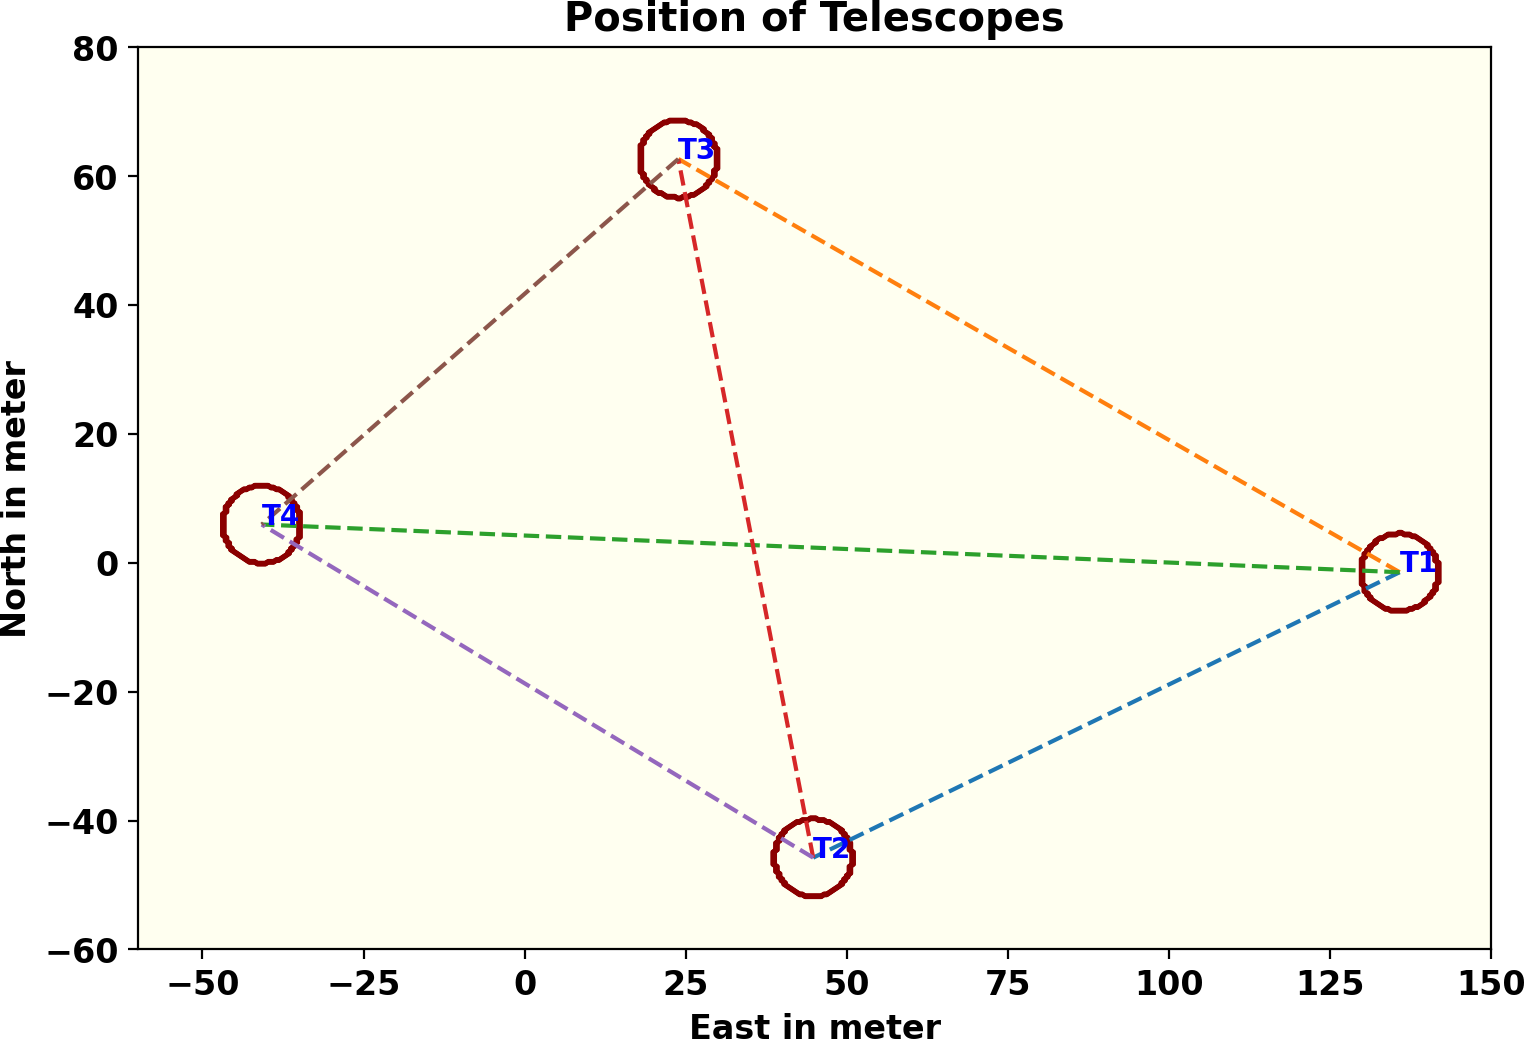
\includegraphics[width=\linewidth]{fig/telescope.png}
	\caption{The telescope configuration with similar properties each, where diameter is 12 meter and baselines are spreaded over more than 100 meter. This setup is used to simulate the signal for II observation.}
	\label{fig:teles}
\end{figure}